\subsection{Data Quality Validation}
The Van Criekinge et al.~\cite{vancriekinge2023dataset} clinical motion capture dataset contains recordings from 138 subjects across the lifespan.
During preprocessing, we resolved dataset-specific artifacts including sensor measurement errors, initialization transients, and mislabeled markers; after discarding 138 T-pose calibration clips, 24 short clips ($<40$ frames), and 4 manually identified artifact clips, the data loader yields 420 effective walking clips (Young 115 / Mid-age 154 / Elderly 151).
To preserve biological fidelity during conversion to the HumanML3D machine-learnable format, we applied a multi-stage optimization procedure adapted from VPoser~\cite{pavlakos2019expressivebodycapture3d}: the optimizer first recovers global body pose, then refines localized artifacts around body shape and limbs.
The fitting loss converges rapidly and eliminates the mesh-inflation and crouch-walking artifacts of Fig.~\ref{fig:artifact}; the converged residual is non-zero, reflecting legacy marker layout and remaining occlusion errors that contribute to the within-group variance visible in our distributional comparisons.

\subsection{Model Training Results}

\subsubsection{ST-GCN Age Representation Learner}
We fine-tuned the ST-GCN++ architecture to classify the processed walking clips into three age categories: Young ($<35$), Mid-age (35--60), and Elderly ($\geq60$).

\begin{figure}[H]
	\centering
	\begin{minipage}[t]{0.49\linewidth}
		\centering
		\IfFileExists{sec/figs/stgcn_train_loss.png}%
		{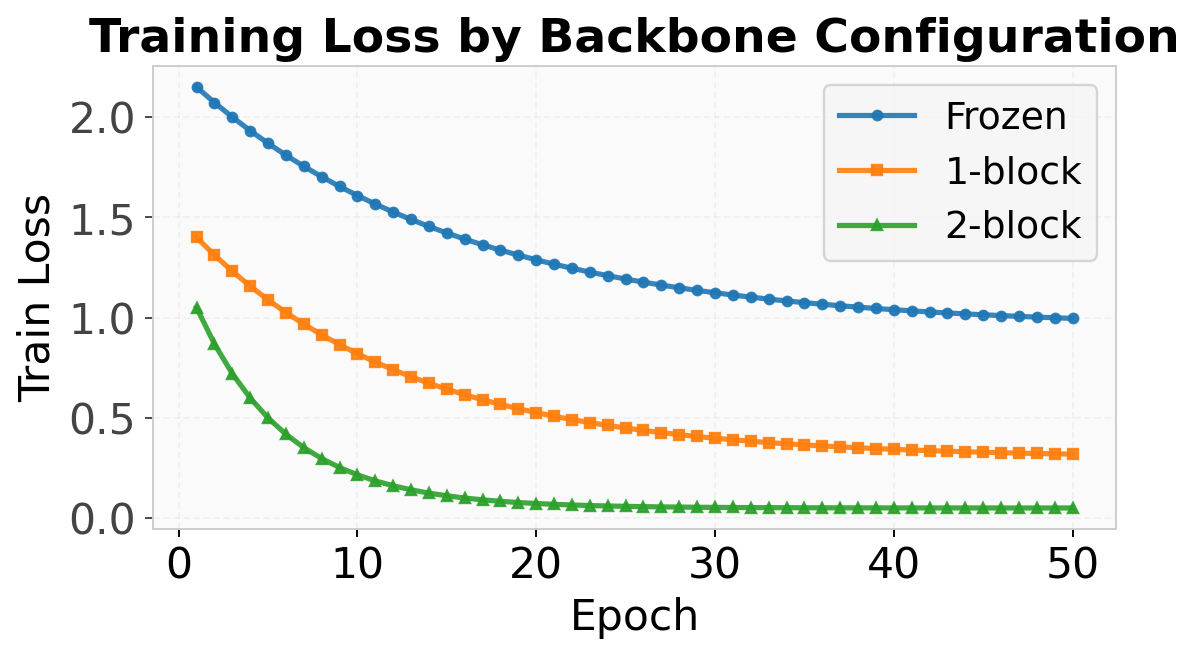
\includegraphics[width=\linewidth]{sec/figs/stgcn_train_loss.png}}%
		{}
	\end{minipage}\hfill
	\begin{minipage}[t]{0.49\linewidth}
		\centering
		\IfFileExists{sec/figs/stgcn_val_accuracy.png}%
		{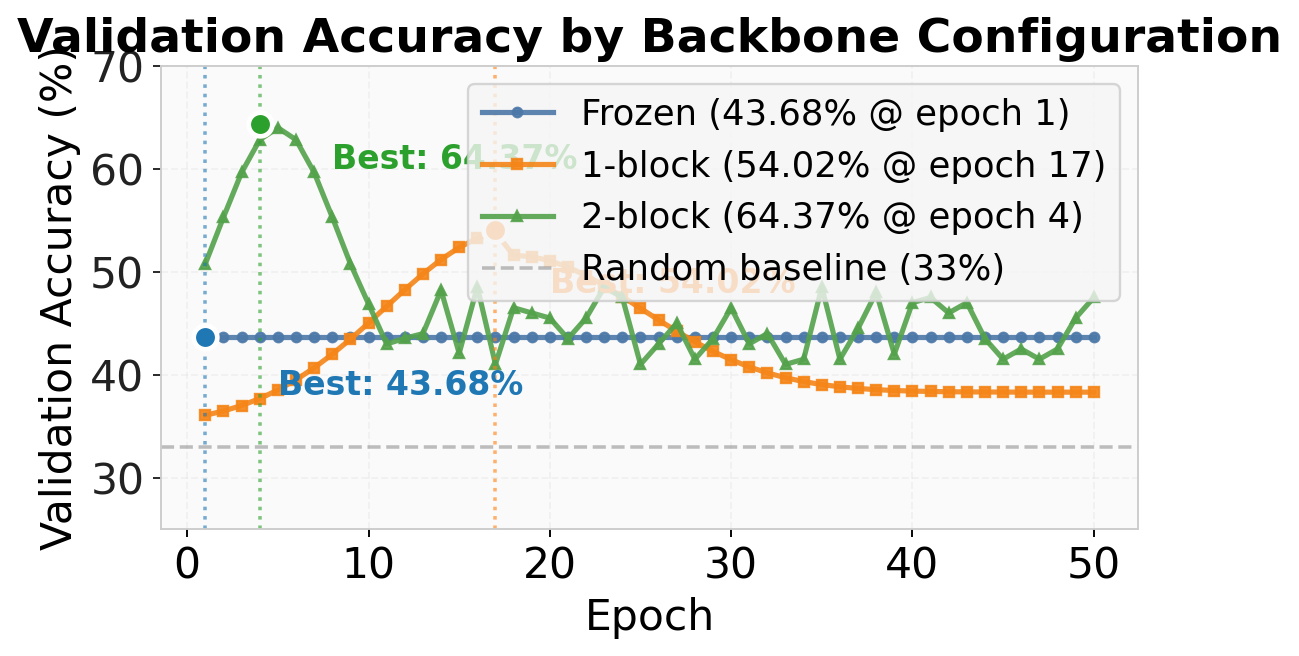
\includegraphics[width=\linewidth]{sec/figs/stgcn_val_accuracy.png}}%
		{}
	\end{minipage}
	\caption{Training dynamics for the ST-GCN age classifier. Left: training loss. Right: validation accuracy.}
	\label{fig:stgcn_curves}
\end{figure}

\begin{figure}[H]
	\centering
	\IfFileExists{sec/figs/stgcn_confusion.png}%
	{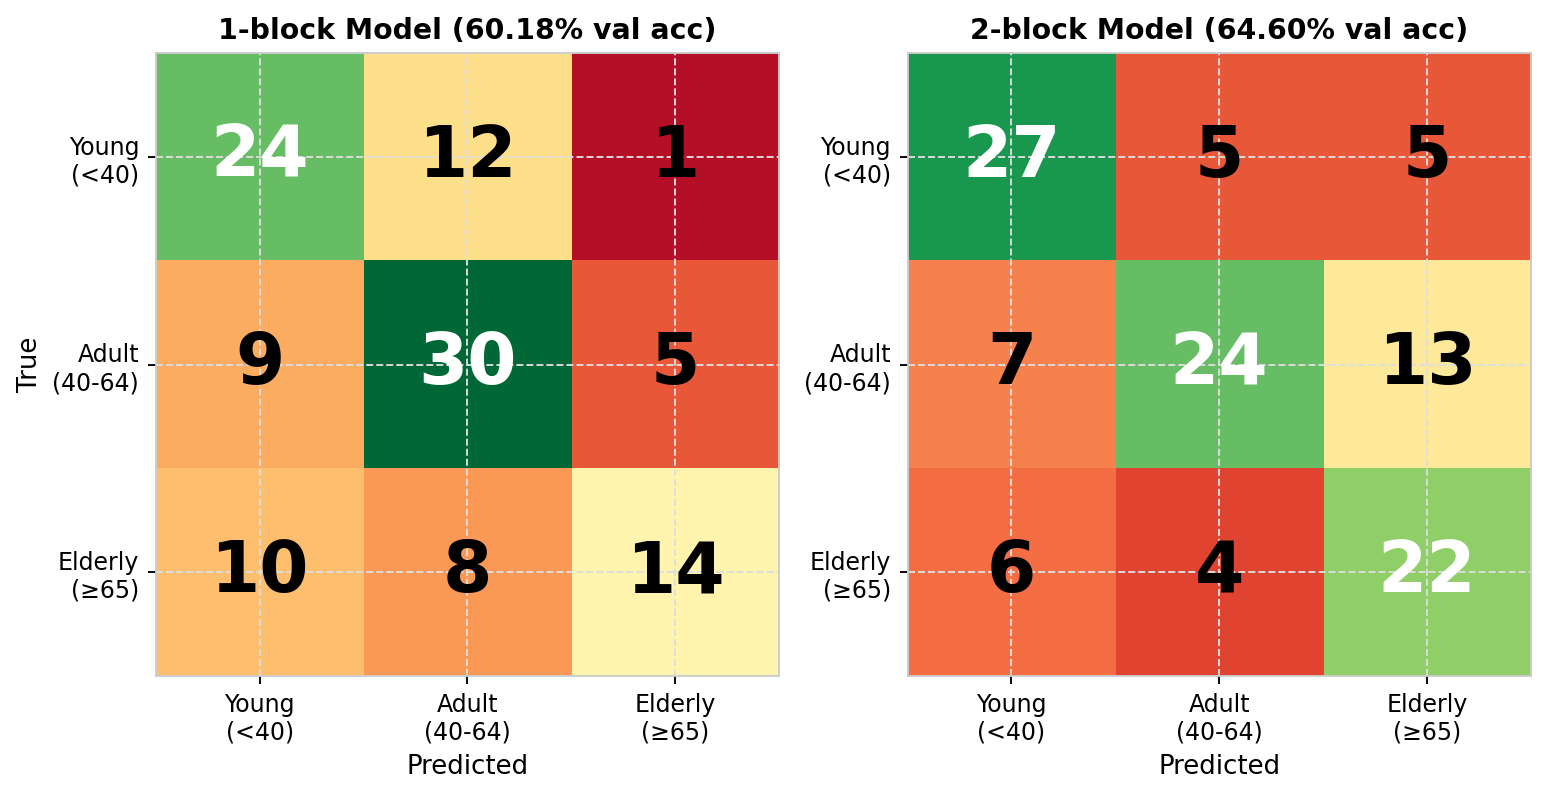
\includegraphics[width=0.8\linewidth]{sec/figs/stgcn_confusion.png}}%
	{}
	\caption{Confusion matrices for the ST-GCN predictions.}
	\label{fig:stgcn_confusion}
\end{figure}

These boundaries are not arbitrary: they roughly balance clip counts across bins and align with clinical findings that the kinematic gap between Young and Mid-age is small relative to within-group variance, whereas distinguishable spatiotemporal decline becomes consistent past 60~\cite{herssens2020investigation}.
To prevent subject-based overfitting --- where the model memorizes individual gait patterns --- we ensured strict, mutually exclusive subject assignment between training and validation, with an approximate 3:1 clip split (315 train / 105 validation clips, subject-disjoint across the 138 subjects).
We progressively unfreeze backbone blocks (Fig.~\ref{fig:stgcn_curves}) to balance validation accuracy (64.60\%) against overfitting, which remains visible as a gap between validation accuracy and the near-perfect training fit.
The confusion matrices (Fig.~\ref{fig:stgcn_confusion}) show that the model consistently separates the kinematic extremes (Young vs. Elderly), with the primary failure mode being the fragmentation of the Mid-age category --- a feature, not only a bug, given the small Young$\leftrightarrow$Mid kinematic gap reported in clinical studies.
We therefore report quantitative trends as Young$\to$Elderly contrasts and include Mid-age as a smooth interior point rather than a hard binary boundary.

\begin{figure*}[!t]
	\centering
	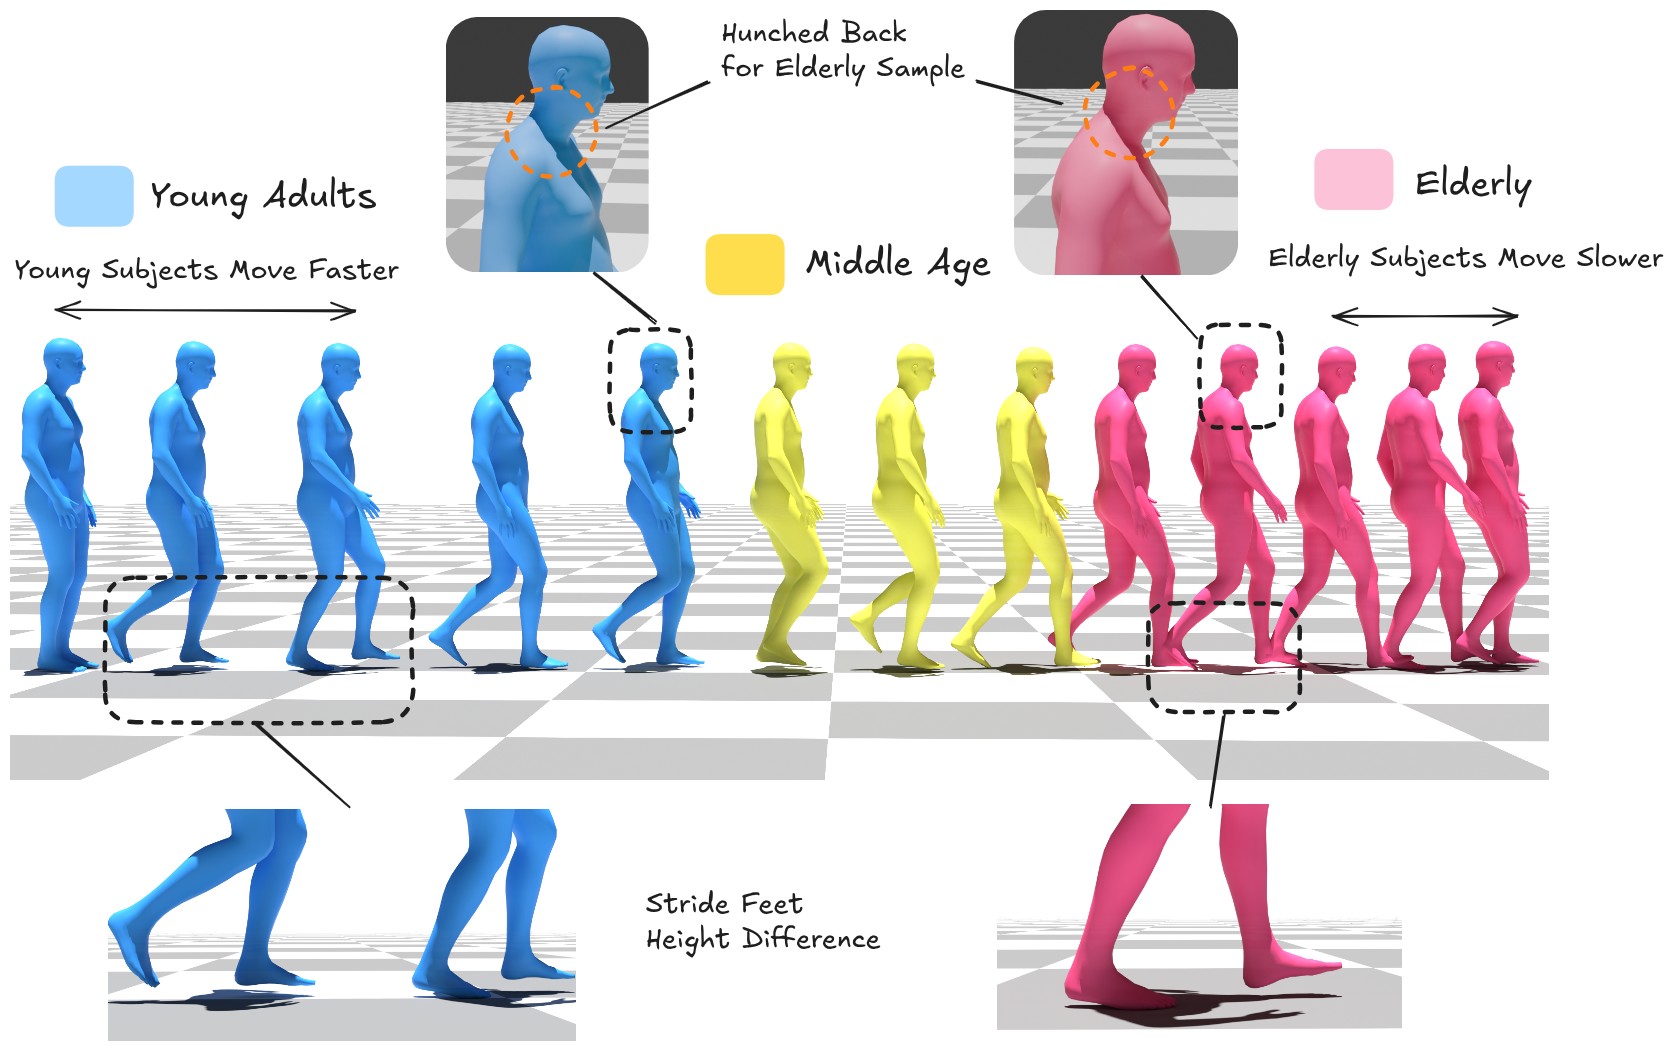
\includegraphics[width=0.7\textwidth]{sec/figs/25 - Generation Result.png}
	\caption{Generated walking sequences across the three age tokens (\texttt{young}, \texttt{mid}, \texttt{old}). The Elderly sample shows a noticeably hunched back and reduced foot-clearance height relative to the Young sample.}
	\label{fig:qualitative}
\end{figure*}
\subsubsection{Generative Motion Synthesis}
As a proof of concept, we conditioned the LoRA-adapted MDM using discrete age tokens.
After training LoRA adapters at ranks 5, 12, and 16, we selected the lowest-loss adapter (rank 12) and generated 3{,}000 clips per age condition (9{,}000 total) from the styled prompt template
\textit{``A person is walking forward in \{\textnormal{young}/\textnormal{mid}/\textnormal{old}\} style''}, with classifier-free guidance scale $s = 1.0$ to remain within the conditional distribution learned during LoRA training.
To isolate the effect of the adapter, we additionally generated baseline clips from the \textit{unadapted} MDM using a neutral prompt \textit{``A person is walking forward.''} and an explicit-age prompt \textit{``An old person is walking forward.''}.

\subsection{Quantitative Clinical Analysis}
We computed standard clinical metrics (Spatiotemporal Parameters, Gait Variability, and Joint Range of Motion) on both the processed ground-truth dataset and the 9,000 generated motion clips.

\subsubsection{Dataset Baseline Validation}
Analysis of the ground-truth dataset confirms that the expected aging signal is preserved end-to-end through our conversion pipeline: monotonic Young$\to$Elderly trends consistent with clinical literature are visible for walking speed, stride length, knee RoM, and stride-time CV (Fig.~\ref{fig:clinical_eval}), and per-clip linear regressions against chronological age (Fig.~\ref{fig:age_regression}) reproduce these directions with weak-to-moderate correlations.

\begin{figure}[H]
	\centering
	\IfFileExists{sec/figs/dataset/age_regression.png}%
	{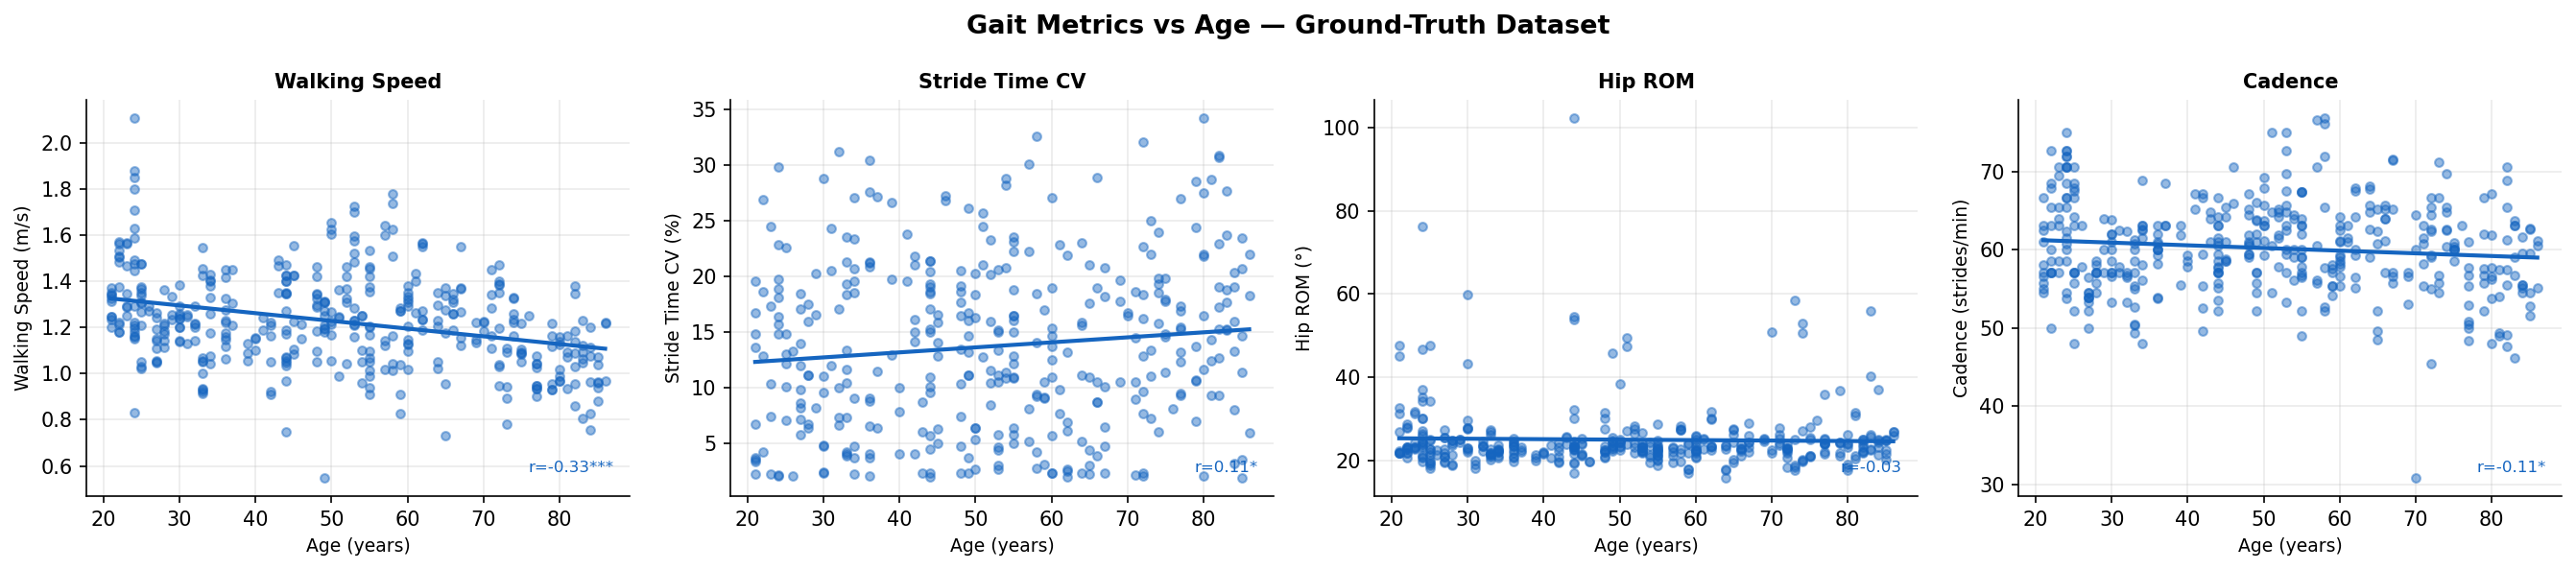
\includegraphics[width=\linewidth]{sec/figs/dataset/age_regression.png}}%
	{}
	\caption{Per-clip linear regression of clinical gait metrics against chronological age on the processed VC dataset.}
	\label{fig:age_regression}
\end{figure}

\subsubsection{Generated Result}
Fig.~\ref{fig:qualitative} shows representative motion sequences generated from the LoRA-adapted MDM under each age token. Coarse stylistic cues of aging are visible: the Elderly sample exhibits a noticeably hunched back, and stride-to-stride foot-clearance height differs visibly between the Young and Elderly conditions. Visual inspection alone is, however, an unreliable proxy for the underlying biomechanics, motivating the quantitative analysis below.

\subsubsection{Quantitative Gait Metrics Comparison}

\begin{figure}[H]
	\centering
	\IfFileExists{sec/figs/combined/combined_violin.png}%
	{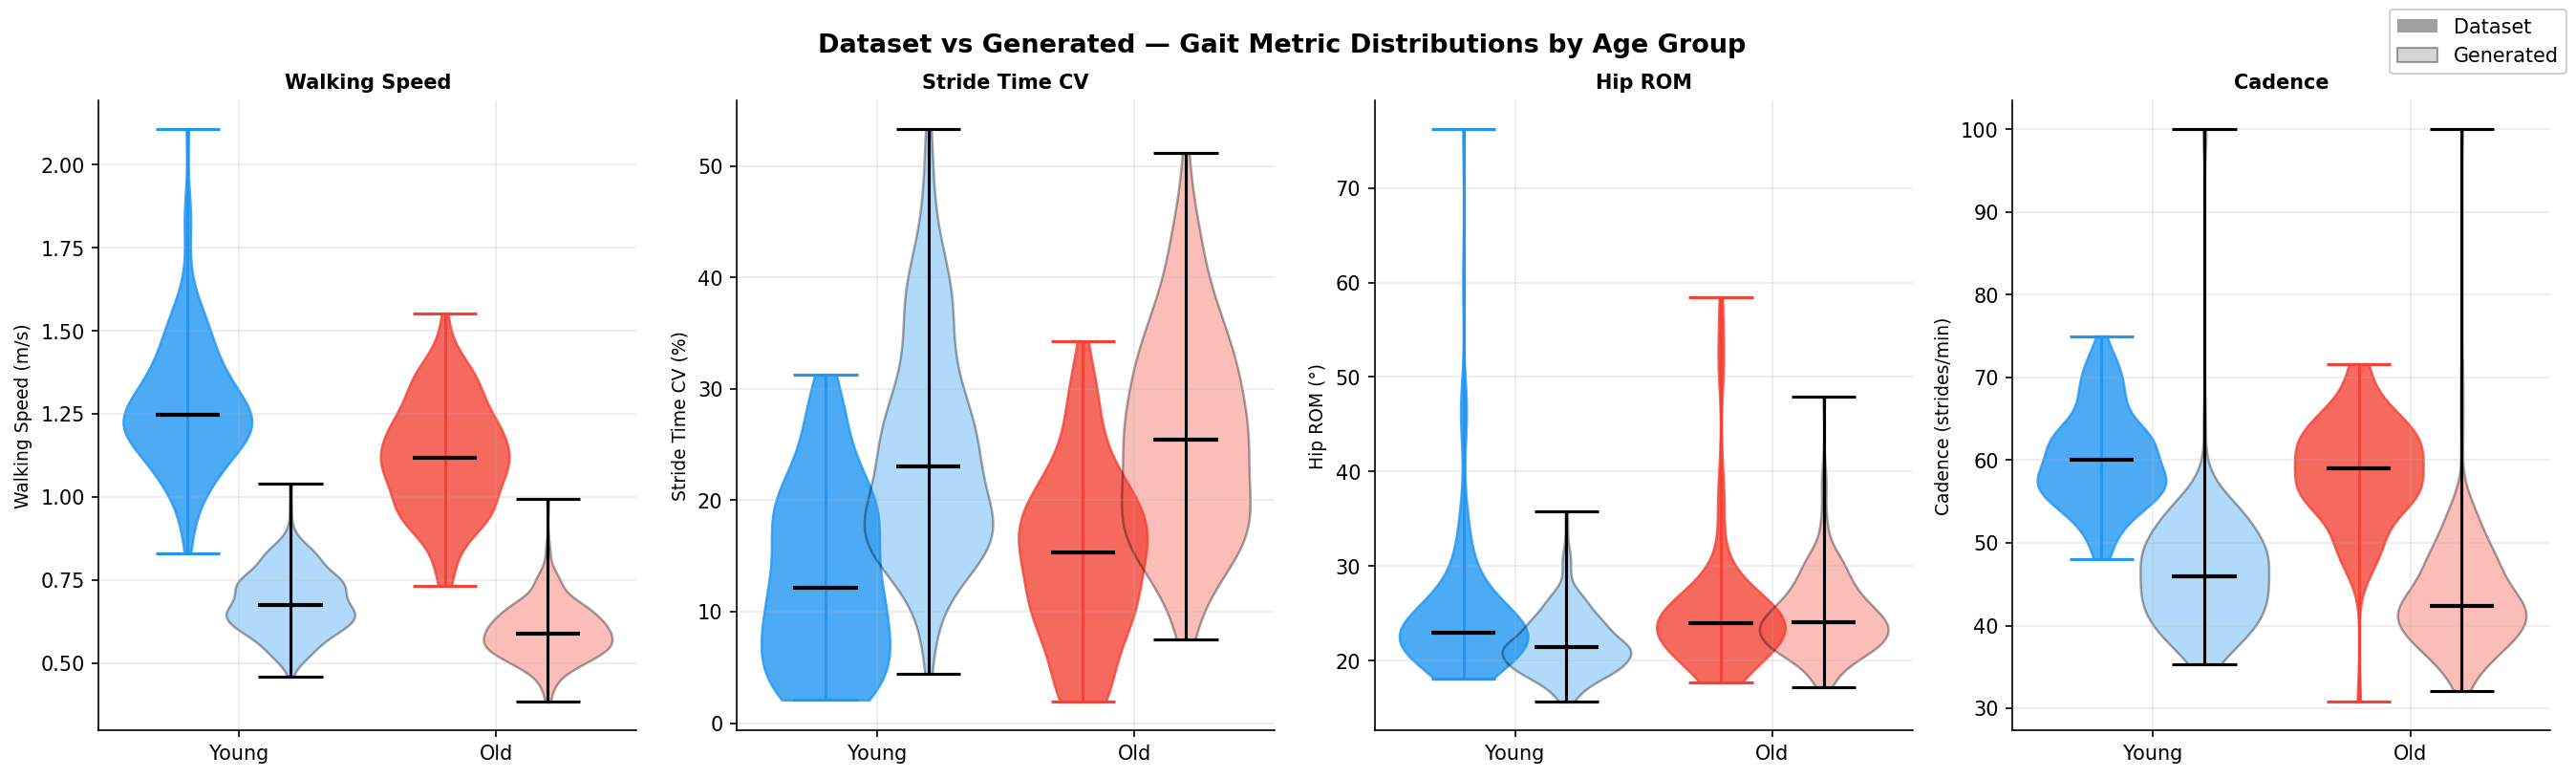
\includegraphics[width=\linewidth]{sec/figs/combined/combined_violin.png}}%
	{\fbox{\parbox[c][2cm][c]{\linewidth}{\centering Plot missing: \texttt{sec/figs/combined/combined\_violin.png}}}}
	\caption{Violin plots comparing the distribution of clinical metrics between the ground-truth dataset and the generated motion clips across age groups.}
	\label{fig:clinical_eval}
\end{figure}

\begin{table}[H]
\centering
\footnotesize
\caption{Welch two-sided $t$-test of Young$-$Old contrast on per-clip metrics at confidence level $\mathbf{C=95\%}$. Values in \textcolor{red}{red} are not statistically significant ($p\!\geq\!0.05$).}
\label{tab:welch}
\setlength{\tabcolsep}{6pt}
\begin{tabular}{lcc}
\toprule
\textbf{Metric (Y$-$O)} & \textbf{Dataset} $\Delta$ & \textbf{Generated} $\Delta$ \\
\midrule
Walking Speed (m/s)     & $+0.155$ & $+0.047$ \\
Stride-Time CV (\%)     & \textcolor{red}{$-1.87$} & \textcolor{red}{$-0.20$} \\
Hip RoM ($^\circ$)      & \textcolor{red}{$-0.25$} & $-0.65$ \\
Cadence (steps/min)     & $+1.61$ & $+1.64$ \\
Joint Lin.\ Vel.\ (m/s) & $+0.140$ & $+0.046$ \\
\bottomrule
\end{tabular}
\end{table}

Table~\ref{tab:welch} reports Welch two-sided $t$-tests of the Young$-$Old contrast on per-clip metrics, on both the dataset and the 9{,}000 LoRA-generated clips. Generated motions reproduce the expected sign and significance for walking speed, cadence, and joint linear velocity; hip RoM becomes significant only in the generated condition ($p\!=\!0.019$), so the adapter sharpens spatial constraints rather than merely mirroring them --- an effect the unadapted-MDM baselines (which fall within the \texttt{young}-token RoM range under both neutral and elderly-described prompts) cannot produce from text alone, confirming that the AMASS prior concentrates on young, healthy actors. Stride-time CV, however, remains non-significant and uniformly elevated (16--19\%) across all generated clips, far exceeding clinical reference values --- a failure we attribute in the Discussion to the capacity ceiling of low-rank, discrete-token adaptation rather than to text conditioning.